One of the main physics goals of the MicroBooNE experiment is to clarify the nature of the low-energy excess of electron-like events observed by the MiniBooNE experiment \cite{Aguilar-Arevalo:2018gpe}. 

However, the MiniBooNE experiment employs a Cherenkov detector, which does not have the ability to distinguish between single electrons and single photons in the final state. This technology limitation makes it very challenging to identify a physics model that could definitely explain the excess.

The MicroBooNE detector, being a LArTPC, provides detailed  calorimetry, which makes it possible to measure the $dE/dx$ of ionisation tracks and electromagnetic showers \cite{Acciarri:2016sli}, and excellent granularity, which allows to measure the gap between the neutrino interaction vertex and the start of the electromagnetic shower. These two methods provide together powerful electron/photon separation and are not normally available in a Cherenkov detector. 

In this chapter we will describe a fully-automated electron neutrino selection using the Pandora multi-algorithm pattern recognition. This is the first fully-automated electron neutrino search in a LArTPC. The selection will be validated with two orthogonal side-bands and with an independent sample of events acquired with the NuMI beam. The systematic uncertainties will evaluated in Chapter \ref{sec:systematics} and the current sensitivity to the MiniBooNE low-energy excess in the electron hypothesis will be estimated in Chapter \ref{sec:sensitivity}.

\section{Signal definition}
The MiniBooNE experiment showed an excess of CCQE-like events in the 200-475~MeV neutrino energy range \cite{Aguilar-Arevalo:2018gpe}, therefore this analysis will focus on a similar topology.

Our selection aims to have a sample with one electron, no other leptons or photons, at least one proton, and no other charged hadrons or mesons in the final state. All particles in the final state are required to be above detection thresholds, measured in Section \ref{sec:eff}. These events are called $\nu_{e}$ CC0$\pi$-Np (where N > 0) \cite{Katori:2013nca}. 

In MicroBooNE, a $\nu_{e}$ CC0$\pi$-Np interaction corresponds to one or more ionisation tracks, produced by the protons, and an electromagnetic shower, produced by the electron. 

The channel closest to the \emph{CCQE-like} events selected by MiniBooNE is CC0$\pi$ (so including events with 0 protons), since the Cherenkov threshold for protons in mineral oil is 350~MeV (kinetic energy) \cite{Perevalov:2009mn}.
However, the choice of the CC0$\pi$-Np channel presents several advantages, described below.
\begin{description}
    \item[Easier pattern recognition.] The presence of a proton in the final state makes vertexing and pattern recognition easier, since there will be typically a \emph{kink} between the ionisation track and the electromagnetic shower.
    \item[Improved energy resolution.] As shown in Section \ref{sec:energyreco}, the length of the ionisation tracks can be used to estimate the energy deposited by the protons. This method provides a higher energy resolution than the one obtained by collecting the deposited charge.
    \item[Improved background rejection.] Requiring an ionisation track allows to reject NC$\pi^0$ e CC$\pi^0$ interactions with no protons in the final state and where one of the $\pi^0\rightarrow\gamma\gamma$ is not reconstructed or escapes the detector. These events represent a large background of our analysis. Also, the presence of the proton allows to reject events with a photon converting far from the interaction vertex, since makes it possible to measure the shower gap.
\end{description}


As an example, figure \ref{fig:evd} shows a simulated $\nu_{e}$ CC0$\pi$-Np event display of the collection plane with an electron and two protons in the final state, with the corresponding reconstructed shower and reconstructed tracks. In this case, the patter recognition is able to correctly identify the electromagnetic shower and both proton tracks.

\begin{figure}[htbp]
	\begin{center}
    	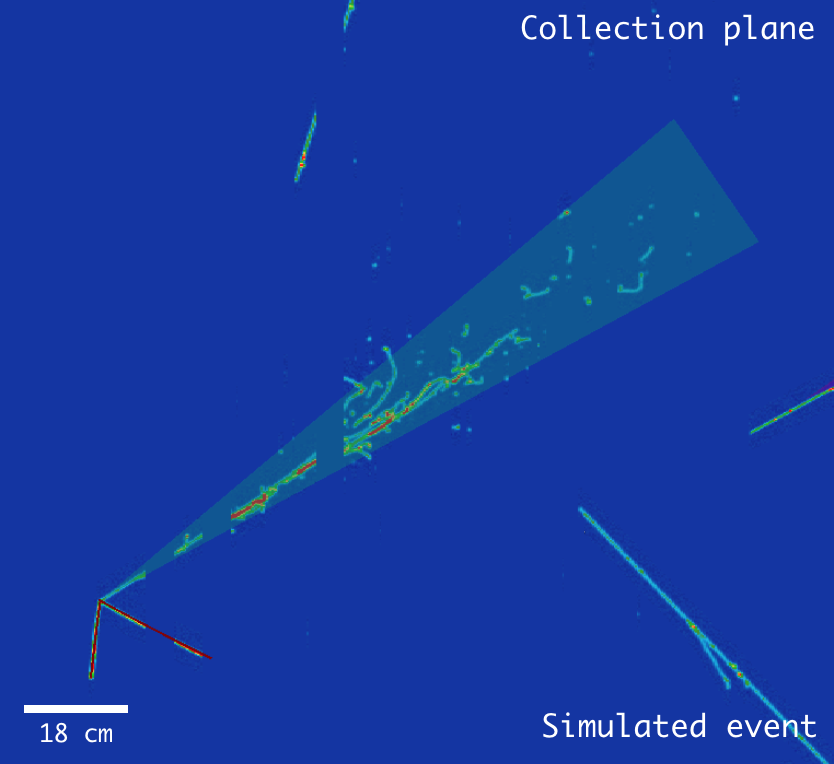
\includegraphics[width=0.85\linewidth]{figures/evd.png}
    	\caption{Monte Carlo $\nu_{e}$ CC0$\pi$-Np event display of the collection plane with an electron and two protons in the final state. The reconstructed shower-like object is represented by the green cone. The reconstructed track-like objects are represented by the red lines. The ionisation trails without an associated reconstructed track are cosmic rays correctly tagged by the cosmic-removal algorithms, described in Section \ref{sec:cosmicremoval}. The colour scale is proportional to the amount of charge collected by the wires. {The vertical gaps are caused by the presence of missing or unresponsive wires in the detector, which are turned off in the simulation.}} \label{fig:evd}
	\end{center}
\end{figure}


